\chapter{Experiment}

\par We carried out an experiment at California Polytechnic State University to test the efficacy of habit-based educational software. We created a web-based application called \textit{Polycommit} that was connected to 4 college classes: \textbf{Introduction to Computer Networks}, \textbf{Introduction to Computer Graphics}, \textbf{Introduction to Computer Networks}, \textbf{Introduction to Operating Systems}, and \textbf{Linear Analysis I}. These classes were selected because they covered subject matter that was easy to convert to online quizzes. For instance, one staple Linear Analysis problem is to find the determinant of a matrix (often a whole number), which is easy to input into an online form. In addition, I had taken these classes in recent quarters and was familiar with the course content. 

\par We presented Polycommit to each of the courses in the first 2 weeks of class. Students voluntarily signed up through a website hosted at https://polycommit.com/, where they were able to log in with one click through the main Cal Poly portal. This lets students easily access the website, while also guaranteeing that only Cal Poly students can sign up for the program.

\section{UI Overview}

\subsection{Home Scren}
\par Upon logging in, students click "Enroll" for the classes they wish to participate in. Upon enrolling, the classes are listed under the "Enrolled Classes" section (\textbf{\hyperref[fig:polycommit1]{Figure \ref*{fig:polycommit1}}}). This page also lists the two main "scores" that students earn by answering questions: \textbf{Commitment} and \textbf{Points}.

\par Commitment is a numerical value that represents how many \textit{unique} days a student has answered a question on the website. Students could earn up to 1\% extra credit on their final grade in the class by getting 15 Commitment.

\par Points are earned by answering questions. More points are awarded for correct answers, and bonus points are awarded based on the user's current Commitment. All participants in the experiment were placed in a raffle for \$20 Amazon gift cards. Additional entries into the raffle were awarded by earning more points.

\begin{figure*}[h]
	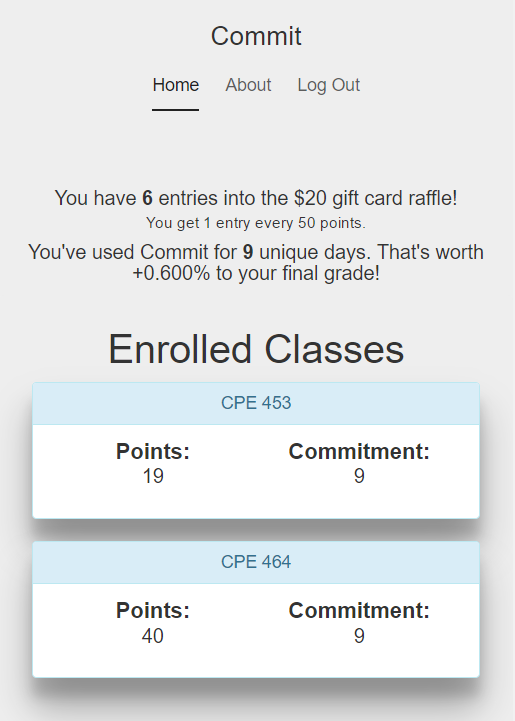
\includegraphics{figures/polycommit-screen}
	\caption{The "Home" screen for Polycommit. Students can see their current progress and can click on a course to answer challenges.}
	\label{fig:polycommit1}
\end{figure*}

\subsection{Course Screen}
\par Each course page has a list of challenges (\textbf{\hyperref[fig:polycommit2]{Figure \ref*{fig:polycommit2}}}) that are open to the student. Challenges are organized into \textbf{Weeks}. If a student has completed all the challenges in a week, the week is displayed with a green check mark and does not expand. If there are open challenges in a week, the week is displayed in yellow with an "alert" icon, indicating that the student has an available challenge. This UI imparts a sense of urgency to the user, since they could potentially lose opportunities to earn Commitment by not answering a question in a . Each challenge also lists the date it was opened, and the number of points awarded if the challenge is already completed.

\par Finally, the Course page lists the student's points and Commitment for the course, along with a tooltip that explains what "Commitment" is. This information is repeated from the Home page, since it is the most relevant information for the user, and it is inherently satisfying to watch your points and Commitment rise as you complete challenges.

\begin{figure*}
	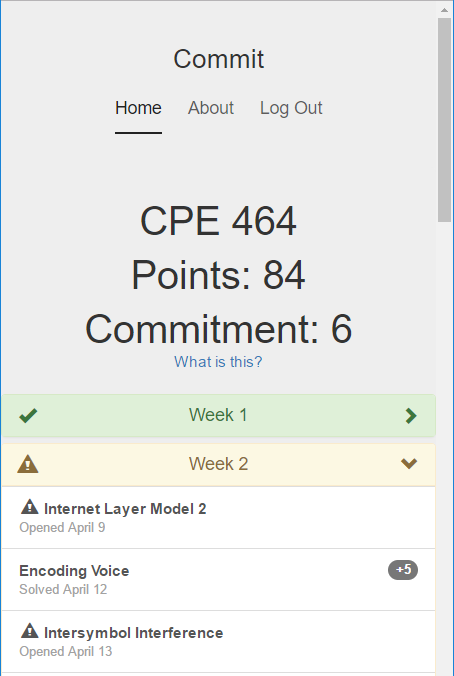
\includegraphics{figures/polycommit-challenges}
	\caption{The "Course" screen for Polycommit. Students can see their current Points and Commitment and can see a list of challenges organized by date.}
	\label{fig:polycommit2}
\end{figure*}

\subsection{Challenge Screen}
\par The challenge screen is where students see the content of a challenge and input their answers. A challenge can either be Multiple Choice, Short Answer, or Numerical. An example of a simple Multiple Choice challenge is at \textbf{\hyperref[fig:polycommit3]{Figure \ref*{fig:polycommit3}}}.

\par At the bottom of the Challenge screen is a link to submit feedback about a question. Through this link, students are brought to a Google form where they can provide feedback about a particular question. The feedback form is viewable at \textbf{\hyperref[fig:polycommit4]{Figure \ref*{fig:polycommit4}}}.

\par Once the challenge is closed, students can see a list of their previous attempts along with the correct answer to the problem. Certain problems have their answers hidden; for instance, all Linear Analysis problems don't show their answers because many challenges on \textit{Polycommit} are directly from the assigned homework. Hiding the correct answer prevents students from quickly inputting a wrong answer to see the homework solutions. Additionally, if a question has received feedback as being confusing, an "Explanation" field provides detailed context about the answer the problem and potential pitfalls (See  \textbf{\hyperref[fig:polycommit5]{Figure \ref*{fig:polycommit5}}}).

\begin{figure*}
	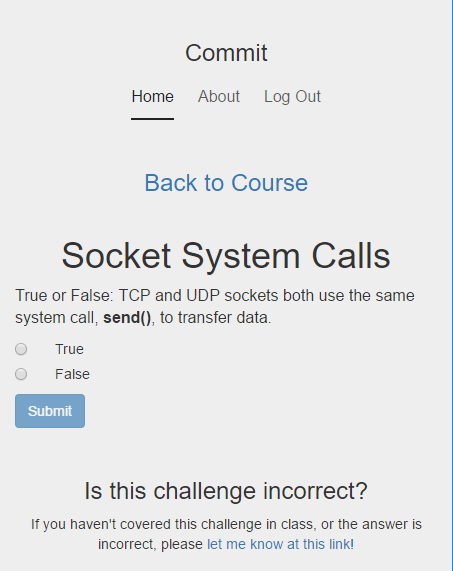
\includegraphics{figures/pc-question}
	\caption{The "Challenge" screen for Polycommit. Students see the content of the challenge and can enter their answers. At the bottom is a link where students can give feedback on a challenge.}
	\label{fig:polycommit3}
\end{figure*}


\begin{figure*}
	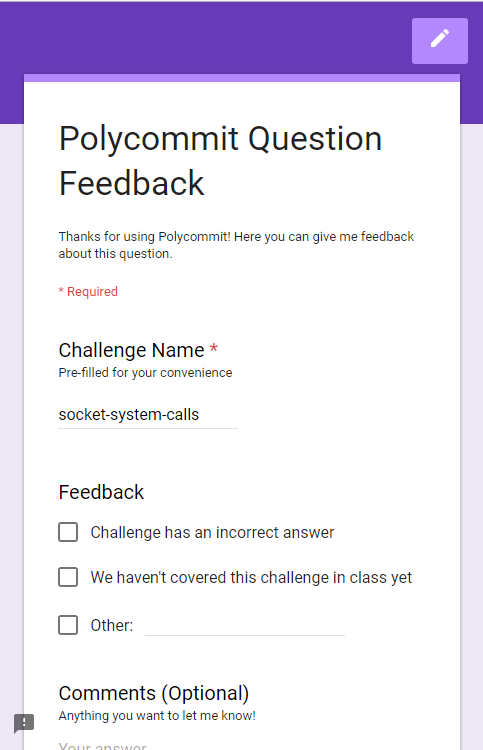
\includegraphics{figures/pc-feedback}
	\caption{The Feedback form for questions. The id for the question is automatically filled in. The student can optionally enter their email address (off-screen) if they want to be contacted when the challenge is fixed.}
	\label{fig:polycommit4}
\end{figure*}

\begin{figure*}
	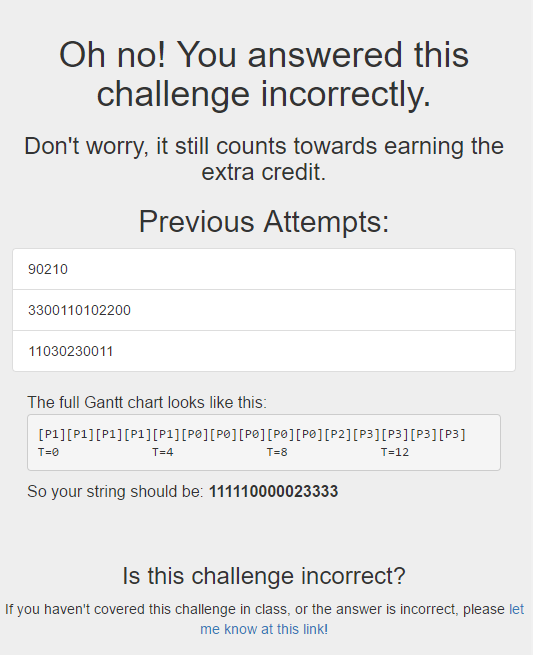
\includegraphics{figures/pc-incorrect}
	\caption{The view of a challenge once it has been answered incorrectly. The main message assures the user that it still counts for Commitment. A full explanation of the problem is under the list of the user's attempts.}
	\label{fig:polycommit5}
\end{figure*}

\subsection{Toasts}
\par \textit{Polycommit} uses "toasts" to convey temporary, state-based information to the user. For instance, when the user answers a question, they get immediate feedback in the form of a pop-up toast. Positive information, such as a correct answer, is styled with a green background and a check mark. Negative information, such as an incorrect answer or a server error, is bright red with an alert symbol that commands the user's attention. Examples of each are at \textbf{\hyperref[fig:polycommit6]{Figure \ref*{fig:polycommit6}}}.


\begin{figure*}
	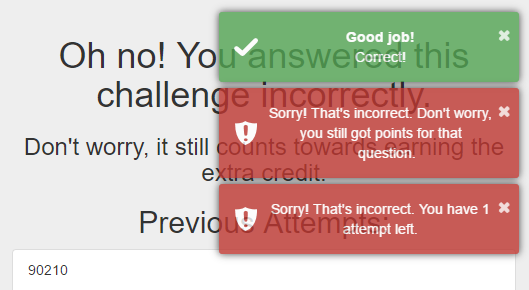
\includegraphics{figures/pc-toast}
	\caption{Three examples of "toast" notifications. These provide useful state-based information, such as whether a challenge was answered correctly. They also can provide feedback if an error occurred, such as a challenge not submitting due to poor network connectivity.}
	\label{fig:polycommit6}
\end{figure*}

\section{Technology Used}
\par All the code for \textit{Polycommit} is available here: 
\hyperref[https://github.com/elliotfiske/commitment]{https://github.com/elliotfiske/commitment}

\par \textit{Polycommit} has its origins in a Summer 2016 section of Dynamic Web Development (CPE 437), taught by Dr. Clint Staley. The base code and overall code architecture remain, as well as some of the platforms used. The app runs on a M*EAN stack. It uses Node.js as a backend, with Express as a routing service and MySQL as a database. In addition, Sequelize is used to easily interface with the database from Javascript. Angular.js is used as a frontend framework, supplemented by Bootstrap for reactive layout.

\par Node.js and Javascript lends itself well to quick, iterative development. As a dynamically typed language with first-class and anonymous functions, it is easy to quickly make sweeping changes based on user feedback. However, since Javascript is an interpreted language, potential errors that a compiler could have caught may make it through to the live site. Because of this, it was extremely important to regularly run the backend code through comprehensive unit tests.

\subsection{Test-First Methodology}
\par All of the backend server code is thoroughly covered by various test cases. I used the service \textit{Postman} to maintain a suite of tests that ensured all the data involved in \textit{Polycommit} was both available and secure. \textit{Postman} allows developers to run a series of web requests against a server, and verify that the correct response or error code is returned (See  \textbf{\hyperref[fig:polycommit5]{Figure \ref*{fig:postman}}}). For instance, one test suite logs in as a student and attempts to complete a challenge, create a class, and query the information of another student. Only the first request should complete successfully; the student's unprivileged account should not be able to create classes or see other students' data.

\par Writing test cases for new server functionality \textit{before} beginning development allowed me to see edge cases before they arose, and allowed for the satisfaction of seeing the tests pass as I completed each feature. In addition, it protected the privacy of students' answers and scores.


%\section{User Feedback}
%Throughout the duration of the experiment, I received a large amount of excellent feedback about the usability of \textit{Polycommit}. At the bottom of each page is a 